\documentclass[english, 10pt]{article}
\usepackage{notes}
\usepackage{turnstile}
\usepackage{qtree}
\usepackage{flagderiv}
\usepackage{pdfpages}
\usepackage{graphicx}

%\renewcommand{\sfdefault}{cmss}
%\renewcommand{\familydefault}{\sfdefault}

\newcommand{\thiscoursecode}{CS34110}
\newcommand{\thiscoursename}{Computer Vision}
\newcommand{\thisprof}{Dr. Hannah Dee}
\newcommand{\me}{Connor Goddard}
\newcommand{\thisterm}{Winter 2014}
\newcommand{\website}{http://connorlukegoddard.com}
\newcommand{\university}{Aberystwyth University}
\newcommand{\feq}{\sdststile{}{}}

%\DeclareTextFontCommand{\emph}{\bfseries}

% Headers
\chead{\thiscoursename}
\lhead{\thisterm}

%%%%% TITLE %%%%%
\newcommand{\notefront} {
\pagenumbering{arabic}
\begin{center}

\textbf{{\Large \noun{\thiscoursecode}}} \vspace{0.2cm}

{\Large{\noun{\thiscoursename}}}\\ \vspace{0.1in}

%\vspace{0in}\includegraphics[scale=0.5]{../logo.png}

  %\includegraphics[scale=0.1]{shield.png} \\
  {\noun \thisprof} \ $\bullet$ \ {\noun \thisterm} \ $\bullet$ \ {\noun \university} \\
  
  {\ttfamily \url{\website}} {\small}

  \end{center}
  }
    
\begin{document}

  \notefront
  
  \tocandfigures
  
% \doabstract{These notes are intended as a resource for myself; past, present, or future students of this course, and anyone interested in the material. The goal is to provide an end-to-end resource that covers all material discussed in the course displayed in an organized manner. If you spot any errors or would like to contribute, please contact me directly.}
%  
%  \hypersetup{linkcolor=black}
  
  \twocolumn
  
  % Turn section numbering back on. 
  \setcounter{secnumdepth}{5}
  
%\section{Introduction}\label{introduction}
%
%  Computer vision is the science of \textbf{\emph{extracting information}} about
%  objects in the 3D-world using noisy, quantised 2D-projections.

\section{Image Formation}\label{image-formation}

\subsection{Geometry of Image
Formation}\label{geometry-of-image-formation}
 
\textbf{ Simple model:} Pinhole Camera (2D-representation of 3D-world)  \\
   
\textbf{Issue}: The distance between the \emph{camera} and the \emph{object} is \textbf{non-recoverable} from a \emph{single viewpoint}.

\subsubsection{Camera Distortions}

\begin{itemize}
  \itemsep1pt\parskip0pt\parsep0pt
  \item
    Limited DoF (Depth of Field = Length between lens and object that is
    in focus - Apeture)
  \item
    Distortions (Lenses have distortion effects)
  \item
    Acqusition speed (Causes image blur)
  \item
    Saturation (Saturated images are those registering at full 255-level
    brightness.)
  \end{itemize}
 
\subsection{Radiosity}

  Brightness at any point depends on:

  \begin{itemize}
  \itemsep1pt\parskip0pt\parsep0pt
  \item
    Amount of light that arrives on surface
  \item
    Amount of light that leaves surface
  \item
    Relative positions of light source and camera plus orientation of
    surface
  \item
    Nature of the surface (matte, mirror etc.) (If the surface is black,
    most of the light will be absorbed.)
 \end{itemize}
 
 \subsubsection{Surface Types}
 
    \begin{enumerate}
    \def\labelenumi{\arabic{enumi}.}
    \itemsep1pt\parskip0pt\parsep0pt
    \item
     \textbf{Lambertian Surface}

      \begin{itemize}
      \itemsep1pt\parskip0pt\parsep0pt
      \item
        Brightness depends only on angle between light and surface
      \item
        Brightness is \emph{independent} of viewpoint.
      \end{itemize}
    \item
      \textbf{Specular Surface}

      \begin{itemize}
      \itemsep1pt\parskip0pt\parsep0pt
      \item
        Brightness depends on angle between light and surface \emph{and}
        \textbf{viewpoint}
      \item
        Light leaves in the same direction as it enters (reflected
        around normal) and doesn't change colour brightness etc.
      \end{itemize}
    \end{enumerate}

\subsection{Digitising}\label{digitising}

  Images do not provide a smooth, continuous representation of the
  world and are composed of a 2D-array of pixel values representing what is
  projected from the world.  \\

 \textbf{Issue: Limited resolution} - Array of \textbf{discontinuous} values causes errors which makes image processing difficult.

\subsubsection{Image Distortion}

  \begin{itemize}
  \itemsep1pt\parskip0pt\parsep0pt
  \item Atmosphere (light, wind, rain etc.)
    \item Acquisition process (lens), 
    \item Acquisition process (sensor)
    \item Quantisation (pixels) and colour quantisation (RGB).
  \end{itemize}

\subsubsection{Colour Spaces}\label{colour-spaces}

\begin{enumerate}
\def\labelenumi{\arabic{enumi}.}
\itemsep1pt\parskip0pt\parsep0pt
\item
  RGB

  \begin{itemize}
  \itemsep1pt\parskip0pt\parsep0pt
  \item
    3 components (RGB) with values between 0-255 (``RGB cube'')
  \item
    \textbf{Not good for CV} - Colour and luminance are tightly linked.
  \end{itemize}
\item
  HSV (Hue Saturation Value)

  \begin{itemize}
  \itemsep1pt\parskip0pt\parsep0pt
  \item
    \emph{Colour} is separated from \emph{luminence} and
    \emph{brightness}.

    \begin{itemize}
    \itemsep1pt\parskip0pt\parsep0pt
    \item
      Hue = Colour (0-360)
    \item
      Saturation = \emph{Quantity} of colour (0-255)
    \item
      Value = Dark to light scale (0-255)
    \end{itemize}
  \item
    Better than RGB.
  \end{itemize}
\item
  CIE L\emph{A}B*

  \begin{itemize}
  \itemsep1pt\parskip0pt\parsep0pt
  \item
    Very good seperation of colour from luminance.
  \item
    \emph{The colour will be the same at different brightness levels}.
  \item
    Luminance is completely seperate to colour shade.
  \item
    Particularly useful for \textbf{shadow detection}.
  \item
    \emph{Requires a colour-calibrated camera.}
  \end{itemize}
\end{enumerate}

\subsubsection{Colour
Calibration/Correction}\label{colour-calibrationcorrection}

\begin{itemize}
\itemsep1pt\parskip0pt\parsep0pt
\item
  We can correct for colour effects caused by the camera as we can know
  what the \emph{real} colour is.
\item
  Normal cameras capture RGB

  \begin{itemize}
  \itemsep1pt\parskip0pt\parsep0pt
  \item
    \emph{Hyperspectral} and \emph{multispectral} cameras capture light
    at particular \emph{wavelengths}.
  \end{itemize}
\end{itemize}

\subsection{Camera Types}\label{camera-types}

\begin{enumerate}
\def\labelenumi{\arabic{enumi}.}
\itemsep1pt\parskip0pt\parsep0pt

\item
  Perspective Projection

  \begin{itemize}
  \itemsep1pt\parskip0pt\parsep0pt
  \item
    Pinhole model uses \textbf{perspective} projection.
  \item
    Perspective projection loses \emph{size} information.
  \end{itemize}
\item
  Parallel Projection

  \begin{itemize}
  \itemsep1pt\parskip0pt\parsep0pt
  \item
    Parallel projection does not lose \emph{size} information, but
    \emph{absolute depth} is lost (Pinhole model with \emph{infinite}
    focal length).
  \end{itemize}
\item
  Omni-directional

  \begin{itemize}
  \itemsep1pt\parskip0pt\parsep0pt
  \item
    Provides 360 degree view from single image.
  \item
    Rotating flat mirror, or fixed hyperbolic mirror (visual compass).
  \item
    Causes \emph{\textbf{distortions}} and \emph{non-homogeneous} resolution
    (parts of the from the compass are higher resolution than others.).
  \item
    Can correct distortion by determining a transformation matrix that
    can balance out the effects of the lens (e.g. Chessboard calibration).
  \end{itemize}
\end{enumerate}

\section{Edge Detection}\label{edge-detection}

  Images are perceived as \emph{\textbf{regions}}. \\

  The regions are surrounded by \emph{\textbf{boundaries}}. \\

  The boundaries are made up of \emph{\textbf{edges}} at the \textbf{\emph{pixel
  level}}. \\

  Edges/boundaries are detected by looking for \textbf{\emph{sharp
  changes in \emph{intensity} between pixels}}. \\
  
   Located by \textbf{\textit{differentiating}} the intensity function once (maxima) or twice (zero crossings).
  
  \subsection{Differentiation}
  
  Gives a good indication of the \textbf{gradient} of a digital function.
  
  $$ f(x) = x_0, x_1, x_2, x_3, ...$$
  
  $$ \frac{df}{dx} \approx \frac{x_2 - x_0}{2}, \frac{x_3 - x_2}{2}, ..., \frac{x_i+1 - x_i-1}{2}$$
  

\subsection{Convolution}\label{convolution}

  We can perform \textit{differentiation} throughout an entire image to look
  for \textbf{very high} (dark-to-light) and \textbf{very low} responses (light-to-dark).\\

  Drag a $[-1,0,1]$ \textbf{mask/kernel} through the image row-by-row whose result is observed to detect edges.

\subsection{First Order Detection}\label{tools}

\subsubsection{Sobel Edge Detector
(1968)}\label{sobel-edge-detector-1968}

  Detects two edge signals at each pixel - one \textbf{vertical} and one
  \textbf{horizontal}. (\textbf{Light} = Low-to-high, \textbf{Dark} = High-to-Low).\\
  
  Addresses two main issues:

  \begin{itemize}
	
  \def\labelenumi{\arabic{enumi}.}
  \itemsep1pt\parskip0pt\parsep0pt
  \item
    \textbf{Noisy edge signals} - Use a 3 x 3 kernel instead of 1 x 3 to provide local averaging effect.
  \item
    \textbf{Looks for both \emph{horizontal} and \emph{vertical} edges} -
    \emph{Use a 3 x 1 kernel as well as a 1 x 3 respectively}.
   \end{itemize}

  Produces an image-sized array of \textbf{\emph{edge strengths}} using
  the formula: $S(x) = \sqrt{S_h(x)^2 + S_v(x)^2}$ where $S_h$ is the horizontal edge, and $S_v$ is the vertical edge. (A \textbf{high value} indicates an edge). \\
  
  Can also calculate the \textbf{direction} of an edge using the
  formula: $\theta(x) = \tan^{-1}S_h(x) / S_v(x)$.

\subsubsection{Canny-Edge Detector
(1986)}\label{canny-edge-detector-1986}

  Utilises (iterated) \textbf{increases} in Gaussian blur and directional first derivative. \\

  \emph{Non-maximal suppression} to suppress \textbf{\emph{thickening}}. \\
  
  Tracking (hysterisis) to link weak evidence to strong. \\
  
  Canny detections at increasing (sigma) Gaussian blur. \\
  
 Two parameters:
 \begin{itemize}
 \item How likely it is to find an edge?
 \item How likely it is to follow the edge once found?
 \end{itemize}

\subsection{Second-Order Detection}

%\subsubsection{Algorithm (General)}
%
%  \begin{enumerate}
%  \def\labelenumi{\arabic{enumi}.}
%  \itemsep1pt\parskip0pt\parsep0pt
%  \item
%    Choose a small sigma ($\sigma$) (used to set the
%    Gaussian ``blurryness'').
%  \item
%    Blur the image with a suitable \textbf{\emph{Gaussian}}.
%  \item
%    Filter with a \textbf{\emph{Laplacian}} (zeroes are the edges).
%  \item
%    Increase sigma and go again to locate \emph{coarser} edges.
%  \item
%    Accumulate \emph{pyramid} of edge detections.
%  \end{enumerate}


\subsubsection{Zero Crossings}

  Provides a powerful mechanism to obtain the \textbf{\emph{location}}
  of an edge within an image.\\
  
  Differentiate the (already calculated) first differential to show a
  sharp ``\emph{up-down signal}'' that \textbf{\emph{crosses zero at the
  edge}}.\\
  
  Issues

  \begin{enumerate}
  \def\labelenumi{\arabic{enumi}.}
  \itemsep1pt\parskip0pt\parsep0pt
  \item
    Directionality

    \begin{itemize}
    \itemsep1pt\parskip0pt\parsep0pt
    \item
      (As with Sobel) we do not know in advance the direction of the
      edges. \textbf{Solution = Laplacian}
    \end{itemize}
  \item
    Noise

    \begin{itemize}
    \itemsep1pt\parskip0pt\parsep0pt
    \item
      Digital approximations to the first ($\frac{d}{dx}$) and second
      ($\frac{d^2}{dx^2}$) derivatives \emph{amplify noise}. \textbf{Solution = Gaussian Blur}
    \end{itemize}
  \end{enumerate}

\subsubsection{Gaussian Blur}
Simulate blurring of images before looking for edges. \\

Allows the \textbf{\emph{strongest}} edges to remain, and the \textbf{\emph{weaker}} edges and \textbf{\emph{noise}} to be \emph{dampened}. \\

Helps to \textbf{\emph{reduce noise}} so the edges are clearer when analysing the derivatives. \\

Applied as a \emph{digital kernel}.

$$ G(x, y) = \frac{1}{2\pi\sigma^2}e^{-\frac{x^2+y^2}{2\sigma^2}}$$

\subsubsection{Laplacian}

Merge of the two second derivatives into \emph{one measure}. \\

\textbf{Zero-crossing of the Laplacian \emph{correspond accurately} to edges.}

$$ \nabla ^2I(x, y) = \frac{\delta {^2}I(x, y)}{\delta x^2} + \frac{\delta ^2I(x, y)}{\delta y^2}$$

\subsubsection{Marr-Hildreth Zero-Crossing Edge
Detector}\label{marr-hildreth-zero-crossing-edge-detector}

\begin{itemize}
\itemsep1pt\parskip0pt\parsep0pt
\item
  Uses Second-Order edge detection by applying \emph{Laplacian} and
  \emph{Gaussian} to image in order to ``block out'' noise.
\end{itemize}
      
\section{Edge Groupings}\label{edge-groupings}

  Take the single pixels extracted (or groups of pixels) from edge
  detection and \emph{group} them into higher-level features/models
  (e.g.~straight lines, curves, blobs, ribbons etc.) \\

  Two main functions of these abstract mathematical models: (cycle between both)

  \begin{enumerate}
  \def\labelenumi{\arabic{enumi}.}
  \item
    \textbf{Distance function} - Measure of how well a given model fits
    the data.
  \item
    \textbf{Search function} - Means of ``wiggling'' model around in
    given space (moving model and re-calculating distance function)
    until the distance goes down to zero.
  \end{enumerate}

\subsection{Edge-Grouping Mechanisms}

\begin{enumerate}

\item \textbf{Edge Following (Bottom-Up)}

\begin{itemize}
 \item
    From an edge pixel, move along the edge direction until the next
    edge pixel is encountered.
\item
  Issues:

  \begin{itemize}
  \itemsep1pt\parskip0pt\parsep0pt
  \item
    Camera/digitisation noise.
  \item
    Gaps.
  \item
    Multiple ``garden paths''.
  \end{itemize}
\end{itemize}

\item \textbf{Projection (Top-Down)}

\begin{itemize}
\item
  A model of what is sought is available and \textbf{\emph{projected}}
  onto the image and matched with the edge pixels.
\item
  Issues:

  \begin{itemize}
  \itemsep1pt\parskip0pt\parsep0pt
  \item
    We need to know what we are looking for (e.g. Person, Car etc).
  \item
    Projection noise.
  \item
    Matching complexity.
  \end{itemize}
  \end{itemize}
\end{enumerate}

\subsection{Line Fitting}

  Finding the line (contour) through a set of pixels using a model in the form: $y = mx + c$ (where $mx$ is the gradient, and $c$ is the intersection with the Y-axis) that \textbf{best fits your model and data}.

\subsubsection{Best Fit}

    Square normals from the proposed line to the point. (Distance
    between line and point ($di$)). 
    
        \begin{figure}[ht!]      
	\centering 
	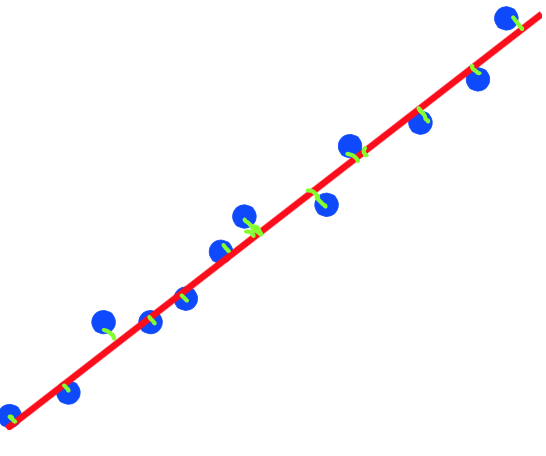
\includegraphics[scale=0.3]{best_fit.png}
\end{figure}

    The best fit will be the line with the \textbf{lowest} total square
    distances from the pixels to that line.
    
\subsubsection{Hough Transform (Finding
Lines)}\label{hough-transform-finding-lines}

\begin{itemize}
\itemsep1pt\parskip0pt\parsep0pt
\item
  Line equation: y = mx + c (Constraints on the line parameters)
\item
  New line equation: xcostheta + ysintheta + r = 0
\item
  All lines going through a pixel create a curve in the \emph{line
  space} of all the line parameters, ``painted'' a \emph{accumulator
  array}.
\item
  Voting from all edge pixels.
\item
  High values in the accumulator indicate lines.
\item
  Can be applied to \emph{other geometrical shapes (e.g.~circles)}.
\item
  \emph{Point where the most pixels vote is the line that is chosen.}
\item
  Pros

  \begin{enumerate}
  \def\labelenumi{\arabic{enumi}.}
  \itemsep1pt\parskip0pt\parsep0pt
  \item
    Good for \emph{geometrical} feature wrapping.
  \item
    Can group widely separated edge pixels.
  \item
    Fast at finding mathematical models in image/pixel data.
  \item
    Easy and fast to find best line via voting mechanism.
  \end{enumerate}
\item
  Cons

  \begin{enumerate}
  \def\labelenumi{\arabic{enumi}.}
  \itemsep1pt\parskip0pt\parsep0pt
  \item
    Can group widely separated edge pixels. (Both a pro and con)
  \item
    Depends on a number of parameters (grid size, threshold) that depend
    on \emph{noise levels}.
  \item
    Needs enough \emph{evidence} to work.
  \end{enumerate}
\end{itemize}

\subsubsection{RANSAC (RANdom SAmple
Consensus)}\label{ransac-random-sample-consensus}

\begin{itemize}
\item
  Least squares fit doesn't always work (i.e \emph{outliers} pull the
  true solution away from \emph{inliers}).
\item
  Process

  \begin{enumerate}
  \def\labelenumi{\arabic{enumi}.}
  \itemsep1pt\parskip0pt\parsep0pt
  \item
    Fit model to a random sub-set of points (sample).
  \item
    Build a \emph{consensus} set: other points that fit the model.
  \item
    Evaluate quality of the model: size and total error of the consensus
    set.
  \item
    \textbf{\emph{Repeat}} steps 1-3 multiple times.
  \item
    Rebuild model with best consensus set.
  \end{enumerate}
\item
  Can estimate no. of iterations needed based on probability of
  outliers, acceptable error and size of samples set.
\item
  Main use at present is for \emph{camera tracking}.
\item
  Like Hough Transform, can be used for more general model fitting (not
  just lines).
\end{itemize}

\section{Feature Detection}

\begin{itemize}
\item
  Detection \textbf{is not} the same as tracking.
\item
  Trade-off between \emph{speed} and \emph{precision}.
\item
  Model-driven (old) - \emph{Brooks etc.}
\item
  Data-driven (new) - \emph{HARRIS/SURF/SIFT etc.}
\item
  A good feature should match the following characteristics:

  \begin{enumerate}
  \def\labelenumi{\arabic{enumi}.}
  \itemsep1pt\parskip0pt\parsep0pt
  \item
    \textbf{Repeatability} - Can it be found easily again?
  \item
    \textbf{Distinctiveness} - Can it be easily separated from other
    areas of the image? (Bricks etc. are not good)
  \item
    \textbf{Locality} - Features should be local (i.e.~not the size of
    the entire image)
  \item
    \textbf{Easy to Find} - Are there enough of them to use for matching
    (Quantity)?
  \item
    \textbf{Accuracy} - Does the feature pinpoint an object/area with
    precision? (Associated more with \emph{feature matching/detection})
  \item
    \textbf{Efficiency} - Can we compute the feature quickly?
  \end{enumerate}
\end{itemize}

\textbf{Features by \textit{their very nature} should be \textit{easy to find again.}}

\subsection{Corner Detection}\label{corner-detection}

\begin{itemize}
\itemsep1pt\parskip0pt\parsep0pt
\item
  Corners are good for finding a common object in multiple images.
\item
  An edge is a place where there is a \textbf{\emph{change in
  intensity}}.
\item
  A corner is a place where \textbf{\emph{edges meet}}.
\item
  A corner can be \textbf{\emph{fast to find}} (like edges, but you're
  probably going to need to look up/down the edge a bit \emph{between
  images}).
\end{itemize}

\subsubsection{Harris Corners}\label{harris-corners}

\begin{itemize}
\itemsep1pt\parskip0pt\parsep0pt
\item
  Don't just look at a patch, look at \emph{neighbours} as well.
\item
  Neighbourhoods of corners are fairly \emph{unique}.
\item
  Harris can be \emph{very fast}.
\item
  \textbf{\emph{Good way of finding objects that are easy to find
  again}}.
\item
  //INSERT HARRIS CORNER FUNCTION
\end{itemize}

\subsubsection{Harris vs KLT}\label{harris-vs-klt}

\begin{itemize}
\itemsep1pt\parskip0pt\parsep0pt
\item
  KLT uses a slightly different \emph{scoring function} to Harris.
\item
  Harris finds more \emph{interest points} than KLT.
\item
  KLT tends to focus more on ``corner-shaped'' parts in the image.
\end{itemize}

\subsection{SIFT (Scale Invariant Feature
Transform)}\label{sift-scale-invariant-feature-transform}

Detects features that are:

\begin{itemize}
\item
  Invariant to \textbf{scale}
\item
  Invariant to \textbf{rotation} in the image plane
\item
  Invariant to small \textbf{translations/rotations}
\item
  Contain a \textbf{local description} of the image
\item
  Used widely in \emph{object recognition}.
\item
  \textbf{\emph{Expensive to run}}, but there are improvements.
\item
  Multiple scales = \textbf{more detections}.
\end{itemize}

\subsubsection{Scale Invariance}\label{scale-invariance}

\begin{itemize}
\item
  Uses a \emph{Gaussian pyramid}:

  \begin{enumerate}
  \def\labelenumi{\arabic{enumi}.}
  \itemsep1pt\parskip0pt\parsep0pt
  \item
    Sub-sampling - Shrink the image by half over and over again to
    produce \emph{pyramid representation}.
  \item
    Gaussian Blur - Blur with different Gaussian kernel widths (make
    less/more blurry) in order to highlight \emph{different features} in
    the image.
  \end{enumerate}
\item
  \textbf{Different detail is highlighted at different levels}.
\item
  Difference between successive images gives the \emph{DoG}.
\end{itemize}

\subsubsection{Feature Selection \&
Localisation}\label{feature-selection-localisation}

\begin{itemize}
\item
  Feature selection is done by using the scale pyramid and the
  difference of gaussians to select features that are \emph{distinctive
  at more than one scale}.
\item
  Features are only selected if they:

  \begin{itemize}
  \itemsep1pt\parskip0pt\parsep0pt
  \item
    Have a \emph{good enough level of contrast}
  \item
    Are on a \emph{corner} (i.e. \textbf{peak of DoG})
  \end{itemize}
\end{itemize}

\subsubsection{Orientation Invariance}\label{orientation-invariance}

\begin{itemize}
\item
  Image gradient computed around each feature at the feature's scale.
  (Using SOBEL edge-detector)
\item
  Feature created for each major orientation (peaks of the 36-bin
  histogram for each feature to represent Gaussian weighted
  orientations) with corresponding orientations.
\end{itemize}

\subsubsection{Feature Description}\label{feature-description}

\begin{itemize}
\itemsep1pt\parskip0pt\parsep0pt
\item
  Image gradient \emph{invarient} to changes in illumination and
  contrast (after normalisation)
\item
  Gradients \emph{grouped} to give some \textbf{\emph{invariance to
  small geometrical transformations}}.
\end{itemize}

\subsection{SURF (Speeded Up Robust
Features)}\label{surf-speeded-up-robust-features}

\begin{itemize}
\itemsep1pt\parskip0pt\parsep0pt
\item
  Sped-up version of SIFT that uses lots of small optimisations.

  \begin{itemize}
  \itemsep1pt\parskip0pt\parsep0pt
  \item
    e.g.~Uses \emph{box features} instead of \emph{LOG filters} (Much
    quicker)
  \end{itemize}
\item
  Used mainly for stereo or feature-tracking.
\end{itemize}

\subsection{Feature Detector
Comparison}\label{feature-detector-comparison}

\begin{itemize}
\itemsep1pt\parskip0pt\parsep0pt
\item
  HARRIS Corner Detector is good for \emph{distinctiveness}.
\item
  KLT tends to go for \emph{distinctiveness} (quality).
\item
  SIFT/SURF tend to go for \emph{``easy to find''} (quantity).
\item
  SURF is \emph{more efficient} than SIFT. Both HARRIS and KLT are also
  fast.
\item
  HARRIS/KLT find \textbf{\emph{corner-like}} structures.
\item
  SIFT/SURF find \textbf{\emph{distinctive regions at multiple scales}}.
\end{itemize}

\section{Feature Tracking}

\subsection{Detection vs Tracking}

\begin{itemize}
\item \textbf{Detection} involves \textit{finding} a particular object/feature within a given image. 
\item \textbf{Tracking} is \textit{monitoring} the movement and detection of the object between multiple scenes.
\item If you have a perfect, fast detector you ``don't need" to track.
\end{itemize}

\subsection{General Framework for Tracking}

\begin{enumerate}
\item \textbf{Model} - We have an idea about how something will change.
\item \textbf{Predict} - We use this to make a prediction.
\item \textbf{Measure} - We measure/see what actually happens.
\item \textbf{Update} - Then update our model accordingly. 
\item \textbf{Repeat.}
\end{enumerate}

\subsection{Advantages}

\begin{itemize}
\item \textbf{Smooths the Data} - Update your estimate of location based upon \textbf{both} the \textit{prediction} and \textit{measurement}.
\item \textbf{Constrains Search} - Use \textit{prediction} to reduce the target search area.
\end{itemize}

\subsection{Issues}

\begin{itemize}
\item \textbf{Initialisation} - If not using detector, where do you start tracking from?
\item \textbf{Multiple Targets} - Multi-target tracking not easy.
\item \textbf{Losing Target} - Losing the target due to objects moving \textit{too fast}, or \textit{drifting off target} or \textit{changing appearance}.
\end{itemize}

\subsection{Kalman Filter (Rudy. E. Kalman)}

\begin{itemize}
\item Well known tracking technique used to find the \textbf{estimate of a moving target}.
\item Once an object starts moving, we expect it to \textit{keep moving} in the \textit{same general direction} and at the \textit{same general speed}.
\end{itemize}

\subsubsection{Advantages}

\begin{itemize}
\item More reliable that just relying on the data, or just relying on the model.
\item Copes with \textit{noise}, \textit{jitter} and \textit{missing information} (e.g. missed detections from face detector etc.)
\end{itemize}

\subsubsection{Tracking Sources}

\begin{enumerate}
\item \textbf{Background subtraction} $\rightarrow$ \textit{Pixels grouped into objects} $\rightarrow$ Tracker
\item \textbf{Sparse Optical Flow} $\rightarrow$ \textit{Features grouped into objects} $\rightarrow$ Tracker
\item \textbf{Face Detection} $\rightarrow$ Tracker
\end{enumerate}

\subsection{Vision Systems}

\begin{itemize}
\item Involve multiple levels.
\item Start with pixels, end up with model of the world (location over time, size, object type, identification).
\item Tracking common when dealing with \textit{motion} and/or \textit{change} (not just $x,y$ data).
\item Can combine \textbf{tracking with detection} (e.g. ``Predator" - TLD).
\end{itemize}

\section{Object Detection}

\subsection{Description}

Does it contain people? $\rightarrow$ Can we find people? (Localisation) $\rightarrow$ Can we group pixels into meaningful classes? (Can we find Connor Goddard?) \\

Applications include \textbf{\textit{face detection}} (People counting, face recognition, face tagging) and \textit{\textbf{self-driving cars}}.

\subsection{Algorithm for Object Detection}

\begin{enumerate}
\item Look at \textit{many} examples of your object (more than one viewpoint). 
\item Represent the examples in some way (i.e. the \textit{\textbf{Model}}).
\item Take the image you are trying to find the object within.
\item Represent this image in some way (i.e. the \textit{\textbf{Image}}).
\item Attempt to find matches between the \textit{model} and the \textit{image}.
\end{enumerate}

\subsection{Elements of Object Detection}

All of the following can have effects on \textbf{robustness} to \textit{variation}, and \textit{efficiency}:

\begin{enumerate}
\item \textbf{Training set} (Many examples of the same object). 
\item \textbf{Representation} (Choice of feature type - (e.g. rectangles with V-J)).
\item \textbf{Model learning} (or calculation).
\item \textbf{Representation of test image(s)}.
\item \textbf{Matching of model to test image(s)}.
\end{enumerate}

\subsection{Representation of Objects}

Linked closely to what makes a \textbf{good feature}:

\begin{enumerate}
\item \textbf{Accessibility} - Can the representation be computed from the image using reasonable resources?
\item \textbf{Scope} - Can the scheme represent a sufficient variety of shapes?
\item \textbf{Uniqueness} - Do two identical shapes have the same representation?
\item \textbf{Stability} - Do two similar shapes have close representations?
\item \textbf{Sensitivity} - So two slightly different shapes differ in their representations?
\end{enumerate}

\section{Object Recognition}

Object recognition is a technique for \textbf{\textit{detecting specific objects}}.

\subsection{Object Detection vs Object Recognition}

\begin{itemize}
\item \textbf{Object Detection} - Modelling \textit{\textbf{within}} class variation. (i.e. ``There is a face in this photo").
\item \textbf{Object Recognition} - Modelling \textit{\textbf{between}} class variation. (i.e. ``This face belongs to Connor.").
\end{itemize}

\subsection{Object Recognition Algorithm}

\begin{figure}[ht!]      
	\centering 
	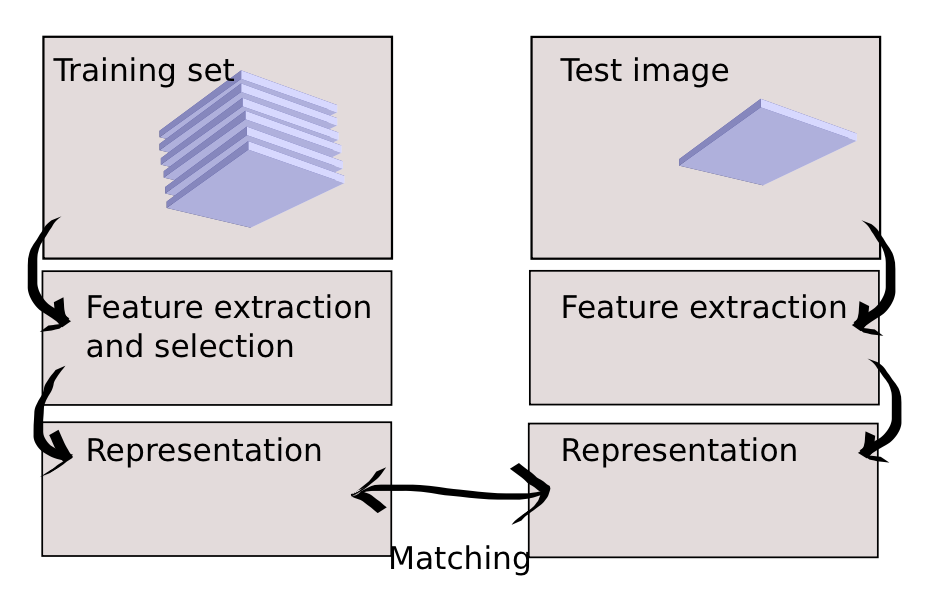
\includegraphics[scale=0.3]{recognition_framework.png}
\end{figure}

\begin{enumerate}
\item Learn a \textbf{model} from image(s) (i.e. large training set). 
\item \textit{Represent} that model in a way that is \textit{easy to search} (e.g. rectangles). 
\item Represent the input in a similar way. 
\item Match input representation to the model representation.
\end{enumerate}

\subsection{Homography}

\begin{itemize}
\item The same scene viewed from \textbf{two different perspectives} results in \textbf{two image planes}.
\item A \textbf{homography} defines a \textbf{\textit{transformation}} relating one set of points on a plane, to the \textit{same} set of points on a different plane.
\item The points will be \textit{noisy}, so we need to fit them to a plane using an \textit{approximation technique} (e.g. \textit{RANSAC}).
\end{itemize}

\subsection{Relationships between Features}

\begin{enumerate}
\item Try to fit feature plane to features in the \textit{current image}.
\item See if they match well to the plane fitted in the \textit{test image}.
\item If so, then we have a match, and object is \textbf{recognised as the same}. 
\end{enumerate}

\subsection{Bag of Words Framework}

\begin{itemize}
\item No order, no structure, just features in a bag. 
\item Requires a training set of \textbf{labelled objects}.
\item Clusters \textit{features} into \textbf{visual words}.
\item Makes \textit{no assumption} about the \textbf{spatial} relationships between clusters (e.g. pile of cow parts, standing on it's head etc.).
\item The model lets the data perform the ``heavy-lifting" to find the features. 
\end{itemize}

\subsubsection{Algorithm}

\begin{enumerate}
\item Large number of features are detected within a large training set (using SIFT etc).
\item \textbf{Cluster} these features based on objects with \textit{similar} appearance being near in \textit{feature space}.
\item For each class of object (e.g. aeroplane, cow etc.) create an \textit{unordered} set of these clusters.
\end{enumerate}


\section{Motion}\label{motion}

Motion is used to detect interesting objects within \emph{video}, and is normally used as a key to other detections (e.g. only detect people where you find motion).

\begin{enumerate}
\def\labelenumi{\arabic{enumi}.}
\itemsep1pt\parskip0pt\parsep0pt
\item
 \textbf{Background Subtraction} - Find objects that \textbf{\emph{aren't
  moving}} and ignore them.
\item
  \textbf{Optical Flow} - Try to find the motion \textbf{\emph{directly}}.
\end{enumerate}

\subsection{Background Subtraction}\label{background-subtraction}

Uses a \emph{static camera} to detect movement in an image. We need to
use a \textbf{threshold} to provide some robustness to noise.

\subsubsection{Simple Background
Subtraction}\label{simple-background-subtraction}

\textbf{Process}

\begin{enumerate}
\def\labelenumi{\arabic{enumi}.}
\itemsep1pt\parskip0pt\parsep0pt
\item
  Take a starting image ($l0$).
\item
  Take another image of the same scene ($ln$) and subtract $l0$ from the image.
\item
  If there is a difference between the background frame and the current
  frame \textbf{\emph{and}} it is greater than the \textbf{threshold}
  ($T$)), then we count it as \textbf{foreground}, otherwise as
  \textbf{background} (Results in a MASK that just contains the parts of
  the second image that are different to the starting image).
\item
  Repeat steps 2-3.
\end{enumerate}

\textbf{Equation}

$$ \| l_n - l_0 \| < T \Longrightarrow Background$$
$$ \| l_n - l_0 \| > T \Longrightarrow Foreground$$

\subsubsection{Moving Average Background
Subtraction}

Moving average background subtraction takes the \textit{mean pixel value over a time window}, and then thresholds on that. \\

Have to account for \textbf{drift}, caused by \emph{lighting},
\emph{sensor noise} etc. in order to prevent \emph{everything} being in
the ``foreground''. \\

Builds a background model which is \textbf{\emph{adaptive}}:

\begin{itemize}
\item
  Deals with \textit{lighting changes}, objects that have been \textit{``put down''} and
  situations where the \textit{scene isn't empty to begin with}.
\item Moving average will \textit{drift} as your lighting \textit{drifts}.  
   \item Otherwise you
  end up with a \emph{change detector}, but not a \emph{motion
  detector}.
\end{itemize}

\textbf{Parameters}

\begin{itemize}
\item
  Threshold $T$ - Determines how likely you are to classify a particular pixel as background.
  
   \item Size of the temporal window - Used to build the background model $w$.
\end{itemize}

\textbf{Equation} \\

Look back through a number of frames (a window, $w$ ), calculate the average image for that window and call it your background $B$, and use that in the subtraction rather than using just one image:

$$ \| l_n - B_{n-1} \| < T \Longrightarrow Background$$
$$ \| l_n - B_{n-1} \| > T \Longrightarrow Foreground$$

Sum up all the images from the current frame looking back $w$ frames from the current frame $n$:

$$  B_{n-1} = \frac{1}{w}\sum_{j=(n-w)}^{n-1}l_j $$

(e.g. Frame 3 will take an average of Frames 1 and 2, and that will then become the background average for Frame 4 etc.)

\subsubsection{Complex Background Subtraction}

\textbf{Flicker}

When investigating single pixels, have to account for \textbf{\textit{flicker}}. Colour of pixel normally varies between a couple of colours. \\

Causes include:

\begin{itemize}
\item Leaves blowing in the wind.
\item Sharp edges in the scene and minor camera shake.
\item TV screens/monitors.
\item Shadows in scene.
\end{itemize}

This makes finding the part of the time-series where the object crosses the pixel much harder.\\

\textbf{Complex Models} \\

Common traits with each model:

\begin{itemize}
\item Each pixel is treated as a \textbf{time-series}.
\item Noise processes are modelled explicitly.
\begin{itemize}
\item Dealing with specific types of noise (e.g. shadow).
\end{itemize}
\item A post-processing step might be used to get rid of small false detections.
\begin{itemize}
\item Simple smoothing, removing detections that are just one pixel .
\end{itemize}
\end{itemize}

Once you have made a decision about what is foreground and what is background, you can use this to update the background model as appropriate. \\

Instead of taking an average of \textit{everything} in the image, we now only update our moving average model with the things in the image that we \textbf{do not} think are moving. \\

\textbf{Complications}

\begin{enumerate}
\item 3D - R, G and B need to be thought about as a single entity (RGB) that \textit{varies together}.
\item Variation \textit{is not constant} - Some objects/noise will vary more than others
\begin{itemize}
\item Simple threshold cannot take this into account.
\item Noise is often Gaussian.
\item Model each pixel as a Gaussian.
\end{itemize}
\item Flicker - The background at a particular place/pixel could be \textit{more than one color}.
\item Gaussian - Determining \textbf{one} Gaussian is easy. Multiple Gaussians requires \textit{machine learning}.
\end{enumerate}

\subsubsection{Mixture of Gaussians Background Modelling (Gaussian Mixture Modelling)}

\begin{itemize}
\item In 2D, a Gaussian is defined by a \textit{mean} and \textit{standard deviation}. 
\item Instead of using a \textbf{\textit{constant threshold}}, use a threshold based on the \textit{\textbf{width of the Gaussian}}.
\item Pixels with a \textit{lot of noise} have a \textbf{\textit{higher threshold}}. 
\item Known also as \textit{Gaussian Mixture Modelling}.
\item Instead of taking one average of the Gaussian model, you take multiple averages. 
\item With three gaussians, we would say each pixel can have up to three different shades of colour in the gaussian.
\item This approach gives a better approach to handling noise when applying background subtraction. 
\end{itemize}

\textbf{Pros}

\begin{enumerate}
\item Deals with complicated backgrounds.
\item Robust to noise.
\item Can handle/detect shadows.
\end{enumerate}

\subsection{Optical Flow}

\textbf{Description} \\

 \textbf{Optical Flow} is the apparent motion of brightness patterns on the image. \textbf{Motion Field} is the projection of objects in the world onto the image plane. \\

\textbf{Issues} \\

Optical Flow is only an \textbf{approximation} of the motion field.

\begin{enumerate}
\item Apparent Motion - When either an object appears to \textbf{not} be moving when it actually \textbf{is}, or vice-versa.
\item Aperture Problem - When you observe a small part of the scene, it is difficult to figure out what motion is occurring. (e.g. ``Barber's Pole" illusion - Motion field is \textbf{horizontal}, but optical flow indicates the stripes move \textbf{vertically}.) 
\end{enumerate}

\subsubsection{Dense Optical Flow}

Designed to show the \textbf{direction of motion} for \textit{every} \textbf{pixel, block or square} in the scene.

\begin{enumerate}
\item \textbf{Appearance-Based } - Looks for movement between pixels in two images and attempts to find the vector between them. 
\item \textbf{Differential Method} (Horn \& Schunck, 1981) - Assume points \textit{between images} will have roughly the same brightness, find nearby points that satisfy this and then calculate the \textbf{direction of travel}. \\ \\ Optical Flow Constraint Equation:  $u\frac{\delta I}{\delta x} + v\frac{\delta I}{\delta y} + \frac{\delta I}{\delta t} = 0 $
\end{enumerate}

\subsubsection{Sparse Optical Flow (Feature Tracking)}

Sparse Optical Flow works by finding the \textit{same feature} throughout multiple images, before calculating it's direction between them. \\

\textbf{Algorithm}

\begin{enumerate}
\item Find features in frame $n$. These become the \textbf{feature set}. (Features in the feature set should be \textit{easy to find again})
\item Find features in frame $n+1$.
\item For each of the features in frame $n$, find the one that \textit{looks most similar} to the feature in frame $n+1$. 
\begin{itemize}
\item If there is no match above a quality threshold, \textit{delete} the feature from the feature set
\item If there is a match, then the \textit{displacement} between the features in the pair of frames is your \textit{motion vector}.
\end{itemize}
\end{enumerate}

\textbf{Speed-ups}

\begin{itemize}
\item \textbf{Assume features do not move very fast} - Constrain the search to a window around the feature.
\item \textbf{Assume features move coherently} - Predict/constrain search in the current direction of motion.
\end{itemize}

\textbf{Advantages}

\begin{itemize}
\item Tracking Ability.
\item Speed.
\item Robustness (Features by their very nature should be easy to find).
\end{itemize}

\textbf{Disadvantages}

\begin{itemize}
\item Tracking Ability - Issue starts if you are wanting to look only for \textit{moving features} - Perform BG subtraction first, then pass into feature detector.
\item Getting Lost (e.g. screen edge, occlusions)
\item Robustness (Features by their very nature should be easy to find).
\item Have to decide where to \textit{re-initialise}. 
\end{itemize}

\section{2D to 3D}

Involves 5 key methods:

\begin{enumerate}
\item \textbf{Shape from Shading} - 1 image, 1 viewpoint, 1 light-source, lots of assumptions.
\item \textbf{Photometric Stereo} - 2+ images, 2+ light-sources.
\item \textbf{Shape from Texture} - 1+ images, lots of assumptions.
\item \textbf{Shape from Motion} - 2+ images, moving objects.
\item \textbf{Stereo Vision} - 2+ images, 2+ viewpoints.
\item \textbf{Depth Cameras} - 2+ images, structured light-source, 1 viewpoint.
\end{enumerate}

\subsection{Shape from Shading}

\begin{itemize}
\item Use the \textit{brightness} properties of an object's surface to gain information about it's \textit{shape}. 
\item Relies on \textit{BDRF} - Defines how a surface interacts with light (fraction of incident light reflected in the direction of the viewer). 
\item Calculates a \textit{reflectance map} that gives the intensity for a given BDRF as a function of surface-orientation \textbf{in gradient space}.
\item Gives us an \textbf{estimate of reflectance}.
\item With one image and one light-source, we can estimate 3D shape:
\begin{itemize}
\item Making assumptions about \textit{smoothness}.
\item Knowing the \textit{reflectance field}.
\end{itemize}
\end{itemize}

\subsection{Photometric Stereo}

\begin{itemize}
\item If we have the ability to re-light the object from \textit{different directions} we can get over \textit{ambiguities}.
\item Use \textit{multiple light sources} to resolve \textit{ambiguity in surface orientation}. 
\item \textbf{Scene does/cannot not move at all}. (Correspondence between points in different images is easy.)
\item Calculates a \textit{reflectance map} that gives the intensity for a given BDRF as a function of surface-orientation \textbf{in gradient space}.
\item Illuminate the object with different lighting patterns (e.g. \textbf{Photometric light-stage}).
\end{itemize}

\subsection{Shape from X}

Add the following techniques to shading (information from light) in order to go to 3D from 2D. 

\subsubsection{Texture}

Determine shape from \textbf{Homogenous} (i.e. texture looks the ``same" everywhere) and \textbf{Isotropic} (i.e. rotation perpendicular to the texture plane does not ``change" the texture) textures. 

\subsubsection{Motion}

Incrementally reconstruction of shape of an object from it's motion as a set of distances between points (e.g. rotating ``dotted" cylinders or ``stickman"). 

\subsubsection{Occlusions}

\begin{itemize}
\item Determine structure from silhouette of objects in scene.
\item  Contours due to discontinuity in depth. 
\item Reconstruction using generalised cylinders (single image) or volumetric reconstruction from several generalised cones (multiple images).
\item 3D scene structure can be inferred by \textbf{motion} and \textbf{occlusion} together.
\end{itemize}

\subsubsection{Focus/Focal Length}

\begin{itemize}
\item Determine shape of scene by calculating distance to objects using \textbf{focal length/aperture}. 
\item Choosing a lens with a \textbf{very narrow depth of field} and varying it. 
\end{itemize}

\subsection{Stereo Vision}

\begin{itemize}
\item Using \textbf{two viewpoints}, determine the depth of a scene (Real-time).
\item Works with a calibrated stereo rig.
\item Gives an \textit{estimate of depth}:
\begin{itemize}
\item \textbf{Sparse}: At features.
\item \textbf{Dense}: At every pixel.
\end{itemize}
\end{itemize}

\begin{figure}[ht!]      
	\centering 
	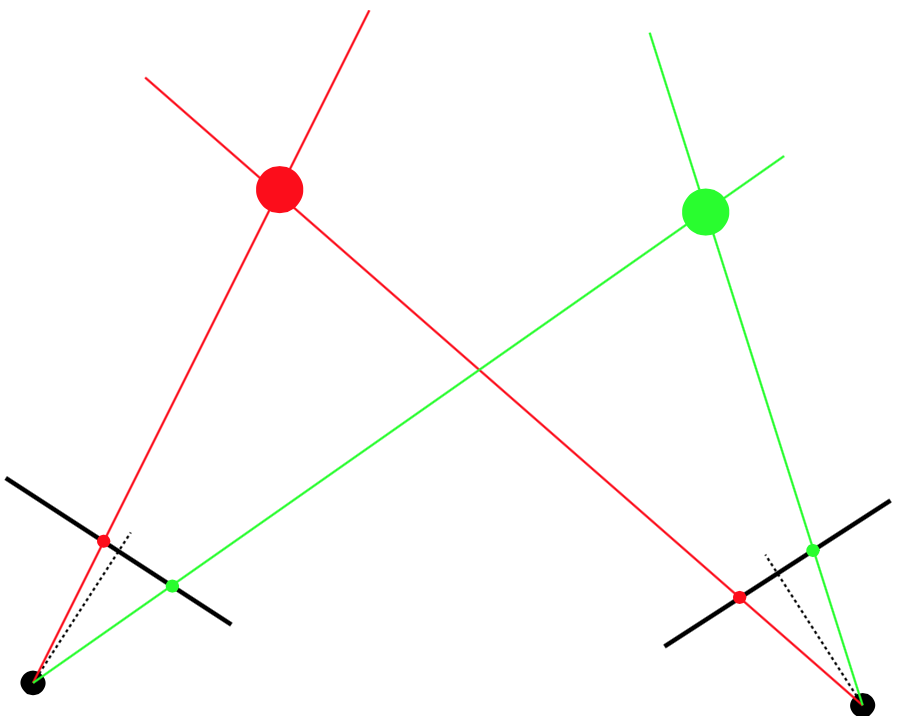
\includegraphics[scale=0.3]{stereo.png}
\end{figure}

\subsubsection{Process}

\begin{enumerate}
\item \textbf{Correspondence Problem} - Finding corresponding points between two images.
\item \textbf{3D-Reconstruction} - Calculating 3D coordinates from \textit{2D image correspondences}.
\end{enumerate}

\subsubsection{Correspondence Problem}

\begin{itemize}
\item Which image entities should be matched? (e.g. area/appearance based, feature-based (SIFT corners), motion-flow)
\item \textbf{Disparity} - Horizontal/vertical displacement between corresponding pixels helps to establish \textbf{scene depth}.
\item \textbf{Issues} - Differences in illumination, specular reflections, lack of texture, occlusions and ambiguity (e.g. repeating structures (e.g. windows) that look the same).
\item \textbf{Multiple Interpretations} - Could be multiple correct matching points. Need to \textit{restrict search}. 
\end{itemize}

\subsubsection{Epipolar Geometry}

Given a point on a line in the \textit{left view}, restrict the search to the \textbf{same line} in the \textit{right view}. 

\begin{figure}[ht!]      
	\centering 
	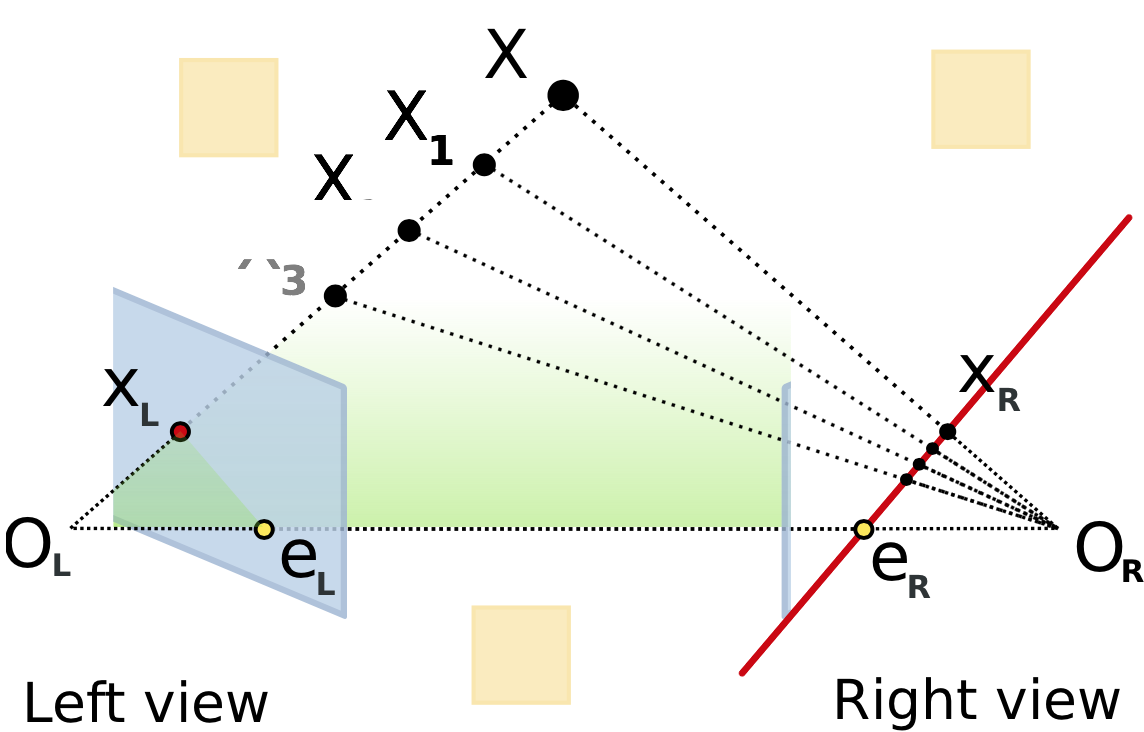
\includegraphics[scale=0.25]{epipolar.png}
\end{figure}

\subsubsection{Depth Estimation}

The \textbf{distance} between two points is \textit{closely linked} to \textbf{depth}. \\

Depth $d$ of point $p$ is given by: $ d = \frac{Bf}{x-x'}$ where $x-x'$ is the \textit{disparity}, $B$ is the distance between the two cameras (baseline) and $f$ is the focal length of the lens.

\begin{figure}[ht!]     
	\centering 
	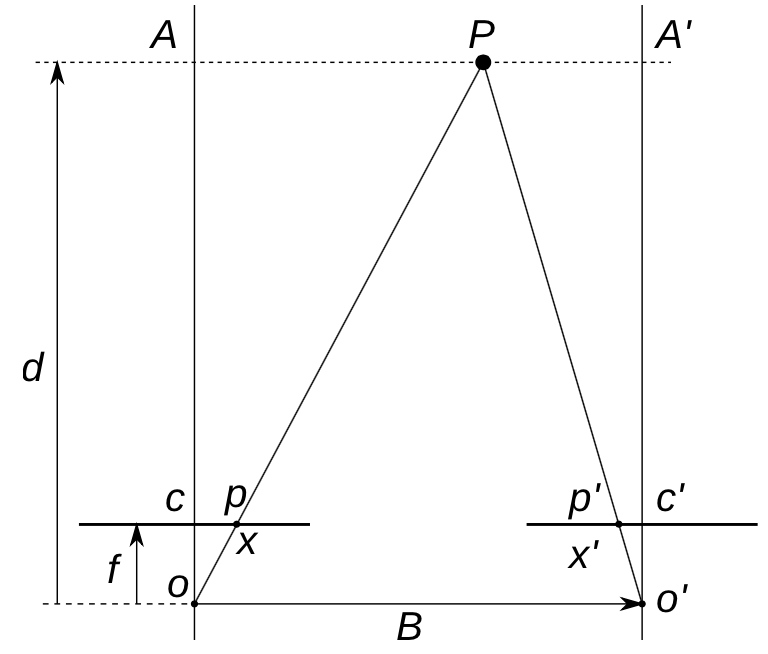
\includegraphics[scale=0.3]{depth.png}
\end{figure}

\subsubsection{Fundamental Matrix}

Fundamental matrix $F$: $x'^TFx = 0$ encodes the geometry of the camera system (i.e. motion between cameras) as a 3x3, rank 2 matrix. \\

Solve for the fundamental matrix given enough matching points between a pair of images. (\textit{More points = less uncertainty}).

\subsection{Structure from Motion}

\begin{itemize}
\item Works with \textbf{uncalibrated} cameras.
\item Gives an estimate of 3D structure (point cloud).
\item Gives \textbf{sparse} structure - Can't work in \textit{real-time}.
\end{itemize}

\subsubsection{SFM vs Shape from Motion}

\begin{itemize}
\item Shape from Motion - Static camera, moving scene/object.
\item Structure from Motion - Moving Camera, static scene/object.
\end{itemize}

\subsubsection{Depth Estimation}

No longer know $B$, \textbf{but} we do know the camera parameters (only have to solve once).

\begin{figure}[ht!]      
	\centering 
	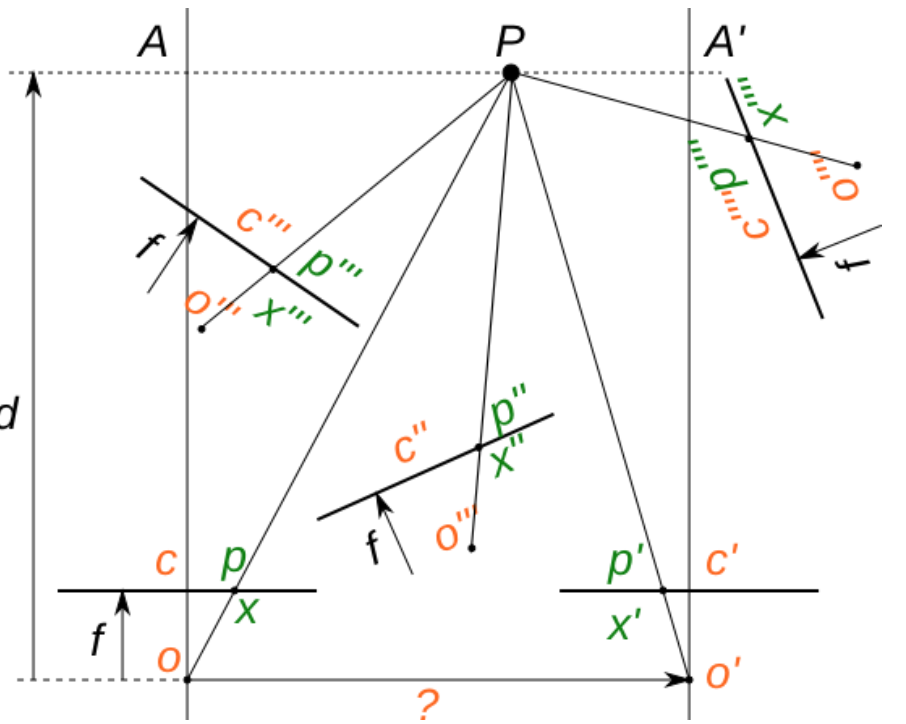
\includegraphics[scale=0.3]{sfm.png}
\end{figure}

\subsubsection{Applications}

\begin{enumerate}
\item \textbf{Camera Tracking} - Calibrating cameras so we know the focal length and camera parameters.
\item \textbf{3D Modelling} - Modelling a scene (e.g. a city) using multiple images from different viewpoints (e.g. \textit{``Bunder"}).
\end{enumerate}

\subsubsection{``Bundler'' Algorithm}

\begin{enumerate}
\item Get a collection of images (various viewpoints).
\item Get information about camera (EXIF).
\item Find features in image (SIFT).
\item Match features between images.
\item Bundle adjustment.
\end{enumerate}

\textbf{Note}: If you have no matches, then you cannot make any assumptions that two images are looking at the same area.

\subsection{Depth Cameras (Active 3D)}

\subsubsection{Methods of Depth}

\begin{enumerate}
\item \textbf{Time-of-Flight} - Time difference. 
\item \textbf{Phased-based} - Check how frequency of wave has changed.
\end{enumerate}

\subsubsection{Range Sensors}

\begin{enumerate}
\item \textbf{Point} - Single point on surface.
\item \textbf{Profile} - Path down or across surface.
\item \textbf{Range Image} - Project a pattern onto surface and observe \textit{warping}.
\item \textbf{Volumetric} - Scan ``slices'' through object (e.g. \textit{MRI})
\end{enumerate}

\subsubsection{Quality Measures}

\begin{enumerate}
\item \textbf{Resolution} - Smallest change in depth that sensor can report? Quantization? Spacing of samples?
\item \textbf{Accuracy} - Degree of conformity of a measured quantity to its actual (true) value. Measurement of what?
\item \textbf{Repeatability (precision)} - Degree to which further measurements show the same result. Do the measurements drift? \textit{warping}.
\item \textbf{Environmental sensitivity} - Does temperature, light conditions or wind speed influence measurements?
\item \textbf{Speed} - Points per second? Seconds per point? Off-line or true real-time?
\end{enumerate}

\subsubsection{Issues}

\begin{itemize}
\item Occlusions
\item Transparent surfaces (can measure \textit{through} glass/ice, but not it itself easily).
\end{itemize}

\subsubsection{Range Data}

Reproduces the 3D structure of a scene. Each pixel expresses the distance of a visible point in the scene from a known reference frame $(i, j, k, x, y, z)$ where $(i, j, k)$ are the coordinates of the \textbf{camera} and $(x, y, z)$ are the coordinates of a point in the world. \\

Represented in two basic forms:

\begin{enumerate}
\item \textbf{XYZ/Cloud Form} - \textbf{Unstructured}, list of 3D coordinates in a given reference frame. 
\item \textbf{RIJ Form} - \textbf{Structured}, matrix of depth values of points along the directions of the $xy$ image axes. Points follow a specific order (given by $xs$ and $ys$).
\end{enumerate}

\subsubsection{Registration}

Range data is \textbf{egocentric} - i.e. has no ``appreciation'' of relationships with other range data. \\

Process of \textbf{joining} multiple scans together to form a single model of the world. \\

Uses \textbf{markers} to join/align \textit{overlapping} images together using \textbf{transformations}.

\subsubsection{Point Clouds}

Triangulate the neighbouring points captured in order to get the surface of the object.\\

\textbf{Convex Hull }- ``Shrink-wrapped" surface around point-cloud. 

\section{Appearance Patches}

Uses \textbf{appearance} over \textbf{geometry} for finding features using \textbf{one or several} images of the objects (at different angles, lighting conditions etc. for \textit{robustness}).

\subsection{Comparing Images}

\subsubsection{Euclidean Distances (Sum of Squared Differences)}

The distance between two points $x$ and $y$ in Euclidean space:

$$ d(x, y) = \sqrt{\sum_{i}\sum_{j}[I(x + i, y + j) - A(i, j)]^2}$$

where $I$ is the whole image, $A$ is the appearance image of the target object ($A$ is always smaller than $I$), $i$ is the current \textbf{horizontal} position, and $j$ is the 
current \textbf{vertical} position. \\

Euclidean Distance is \textbf{not normalised} (issue with variations in brightness). \\

Calculate SSD by removing the square root.

\subsubsection{Correlation Coefficients}

Based on Euclidean distance, but \textbf{independent of overall brightness} (plus small robustness to \textit{noise} and \textit{partial matches}). \\

Euclidean Distance is \textbf{faster} though.

$$ r(x, y) = \frac{\sum{i}\sum{j}[I(x + i, y + j) - \overline{I}(x, y)][A(i, j) - \overline{A}]}{\sqrt{\sum_{i}\sum_{j}[I(x + i, y + j) - \overline{I}(x, y)]^2\sum_{i}\sum_{j}[A(i, j) - \overline{A}]^2}}$$

where $\overline{A}$ is the \textit{average} appearance image and $\overline{I}(x, y)$ is the image ``under'' appearance, $x, y$ in size of $I$ and $i, j$ in size of $A$. \\

\textbf{Threshold} on $r$ can be used: $-1 \leq r(x, y) \leq 1$, high if \textit{good match}, low if \textit{poor match}.

\section{Systems \& Evaluation}

\subsection{Approach Testing}

Computer Vision approaches follow a similar pattern:

\begin{enumerate}
\item Start with an image (e.g. photo, video, point cloud, depth map, MRI scan etc.).
\item One or more processes are applied to the image:
\begin{itemize}
\item Image processing steps (e.g. noise reduction).
\item Intermediate level conversions and representations (e.g. feature extraction).
\item Higher-level vision (e.g. object detection).
\item Maybe even ``higher'' level methods (e.g. semantic information).
\end{itemize}
\end{enumerate}

\subsection{Testing Issues}

\begin{itemize}
\item Separation of training sets and test sets.
\begin{itemize}
\item \textit{Train on 9 out of 10 objects, and test on 10, then train on 8 and test on (9 and 10), then test on 7, and test on (8, 9 and 10) etc.}
\end{itemize}
\item N-Fold validation.
\item Careful design of evaluation scenarios and datasets.
\end{itemize}

%\subsection{Comparison of Techniques}
%
%\begin{itemize}
%\item Use of \textit{shared, open datasets}.
%\item Performance statistics which \textit{use the appropriate/correct} measures.
%\end{itemize}

\subsection{Datasets}

Datasets allow you to \textbf{define the tests before development (like TDD)}. It is important that the datasets have \textbf{enough variation} to give \textit{sufficient testing} (e.g. variation in pose, lighting, orientation etc.)

\subsubsection{Ground Truth}

Describes the ``proper'' data for a particular training \textbf{dataset} (i.e. what an algorithm should \textit{actually} be looking for) (e.g. ``there are 10 faces in this image''). \\

Can be obtained via a number of sources:

\begin{itemize}
\item \textbf{Hand-labelled} - Often by more than one person.
\item \textbf{Acquisition Process} - (e.g. Deliberately  capture $N$ people walking down a known path).
\item \textbf{Different Measurement System }- (e.g. Evaluate a visual tracking system using \textbf{RTK-GPS}).
\item \textbf{Bootstrapped} - Using \textit{informal} ground truths (e.g. social network tags used to train a face recogniser). 
\end{itemize}

\subsection{ROC (Receiver Operating Characteristic)}

Allows visualisation and comparison of YES/NO classifier performance (of the system as a \textbf{whole}). 

\begin{figure}[ht!]      
	\centering 
	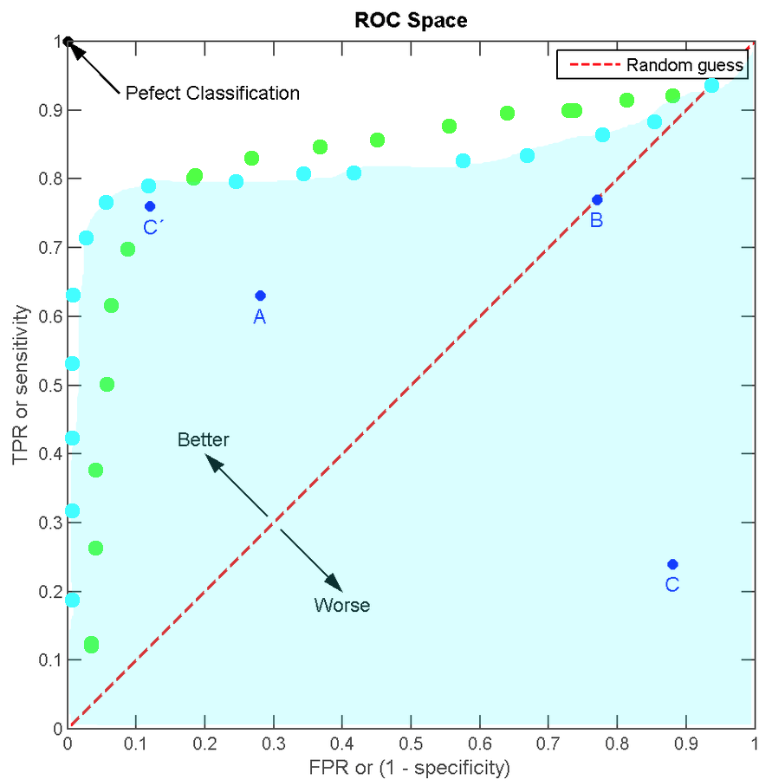
\includegraphics[scale=0.3]{roc.png}
\end{figure}

\subsubsection{AUC}

The Area Under Curve is equal to the probability of a classifier ranking a (randomly chosen) positive instance higher than a (randomly chosen) negative instance. \\

The \textit{higher the area under the curve}, the \textit{higher performance the of the detector} (more TPR and less FPR).

\subsection{Confusion Matrices}

Describes the performance of a \textbf{classification/categorisation} system. \\

Predicted truth along the X-axis, ground truth along the Y-axis. Diagonal is the \textit{correctly-predicted} value.

\begin{figure}[ht!]      
	\centering 
	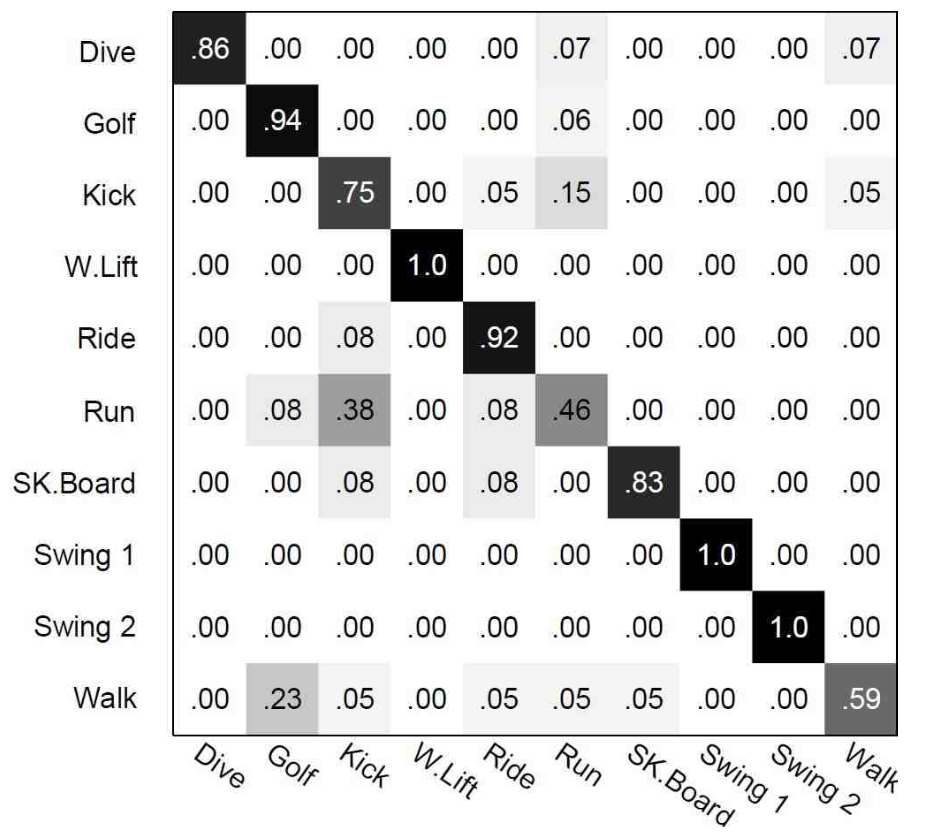
\includegraphics[scale=0.3]{confusion_matrix.png}
\end{figure}

\subsection{Report Measures}

\subsubsection{TPR \& FPR}

\begin{itemize}
\item \textbf{True Positive} - Is a dog, and identified as a dog. 
\item \textbf{False Positive} - Is a cat, but identified as a dog. 
\item \textbf{True negative} - Is a cat, and identified as a cat (and not a dog).
\item \textbf{False negative} - Is a dog, but identified as a cat (should be a dog).
\end{itemize}

\subsubsection{Points \& Lines}

Use the \textbf{mean square error}, that allows measurement of the absolute distance over a set of points. 

\subsubsection{Areas}

For area measures, you can use \textbf{bounding box overlap}:

$$Min = \frac{area(A \cap B)}{min(area(A), areas(B))}$$

or \textbf{bounding box union}:

$$Union = \frac{area(A \cap B)}{area(A \cup B)}$$

\end{document}